\documentclass[a4paper]{article}

\usepackage[left=5mm,right=5mm,top=8.5mm,bottom=8.5mm]{geometry}
\pagestyle{empty}
\usepackage{tikz}
\usetikzlibrary{
    decorations.markings,
    decorations.pathmorphing,
    decorations.text,
}
\usepackage{eucal}
\usepackage{contour}
\contourlength{0.05mm}
\usepackage{fontspec}
\newfontface\textlino{QTLinoscroll}
% \usepackage{yfonts}
% \usepackage{dozenal}
        

\newcommand{\insR}{8mm}
\newcommand{\midR}{20mm}
\newcommand{\outR}{67mm}

\begin{document}
\begin{center}
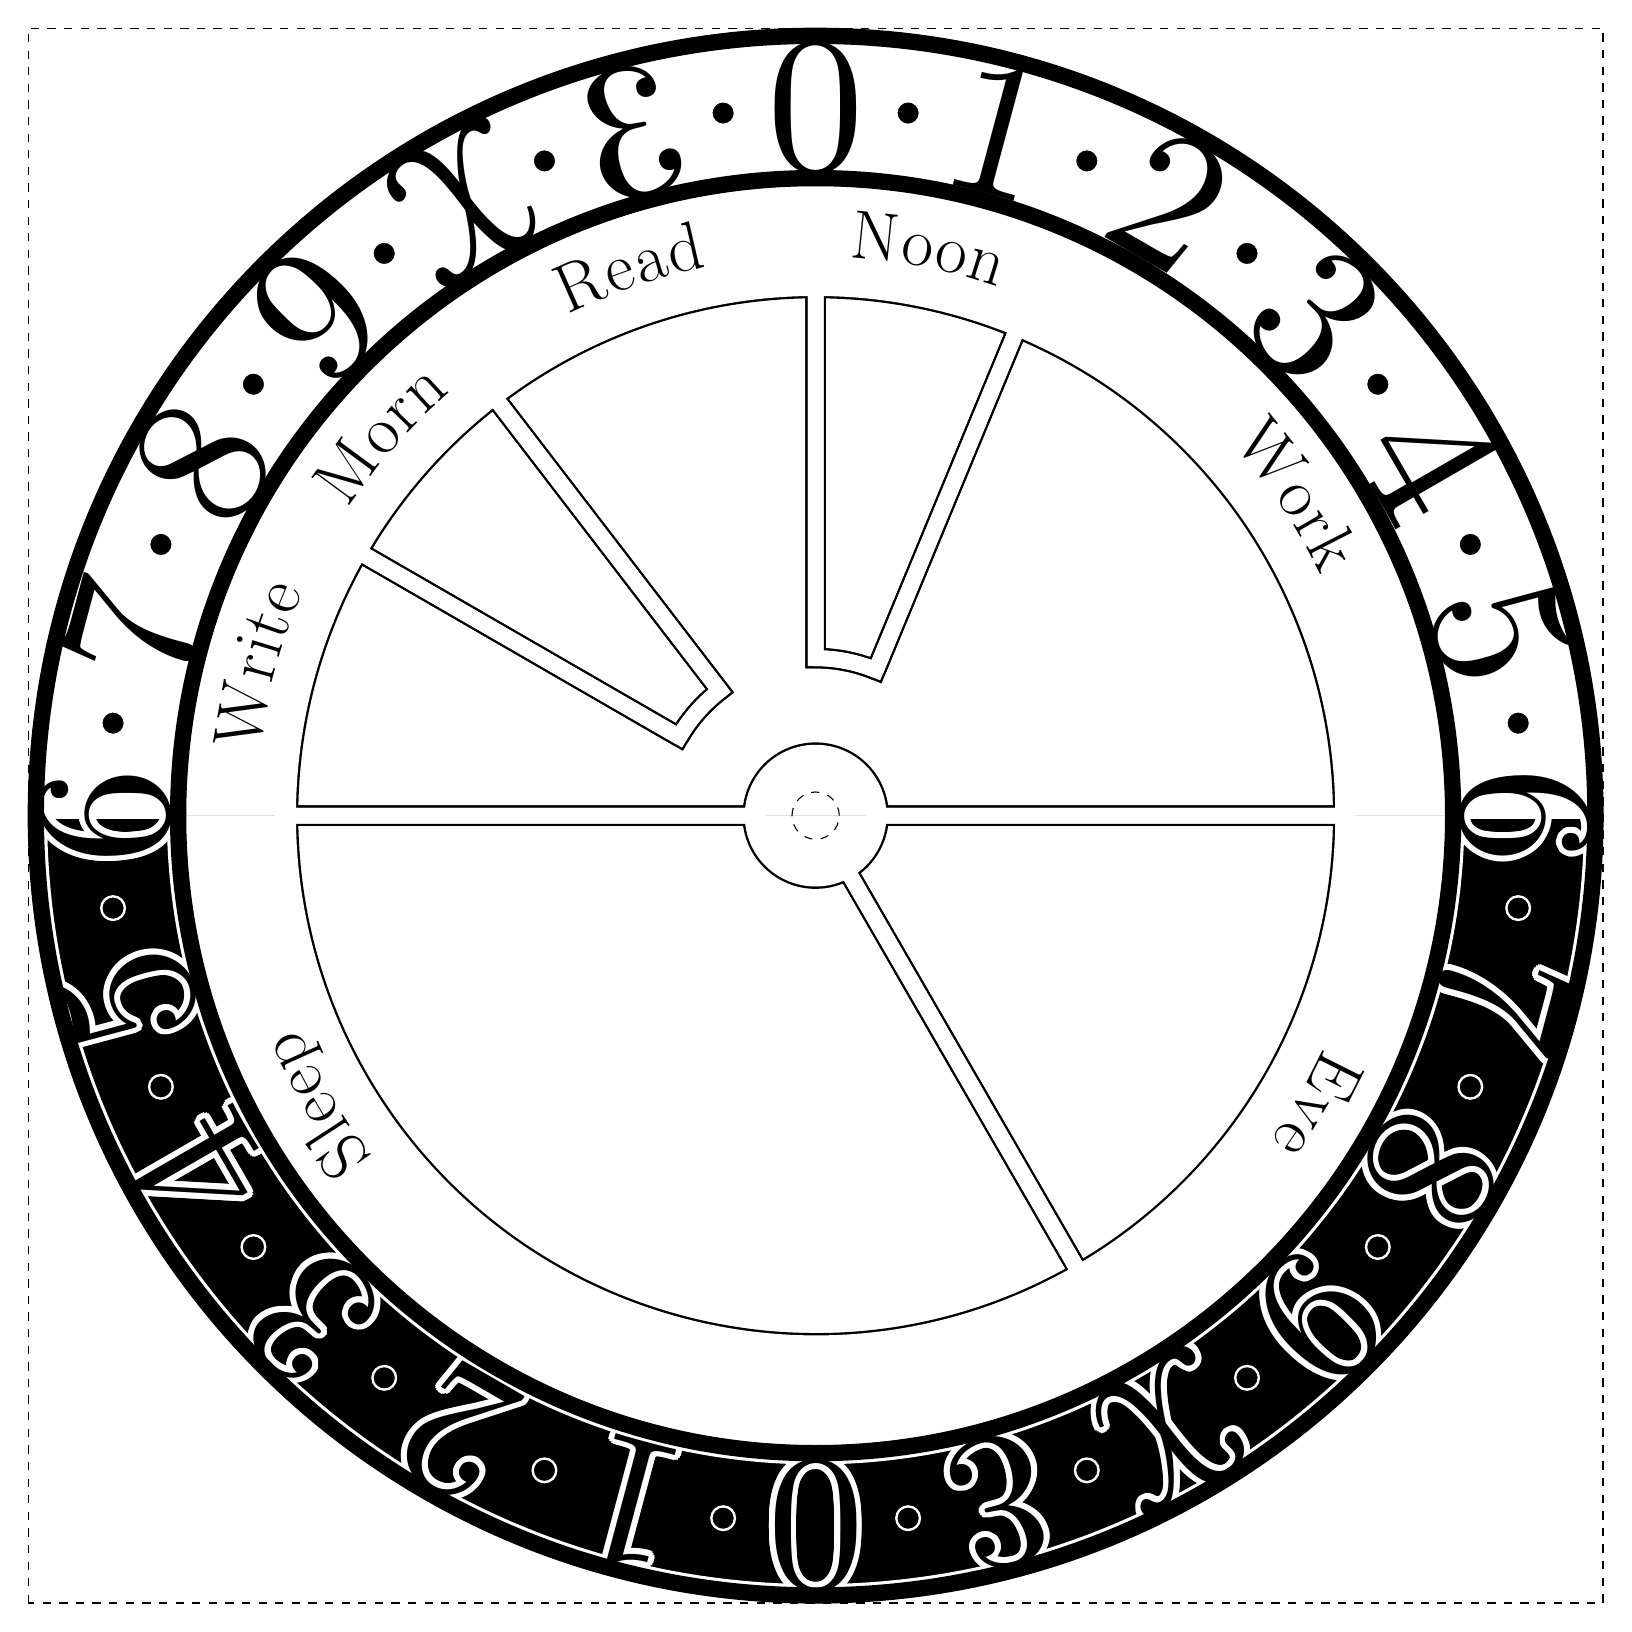
\begin{tikzpicture}
    % BORDER
    \draw[dashed] (-100mm,-100mm) rectangle (100mm,100mm);
    \draw[dashed] (0,0) circle [radius=3mm];

    % SECTIONS
    \draw (0,0) circle [radius=100mm];
    \draw (0,0) circle [radius=80mm];
    
    % NUMBERS
    \draw[fill=black,draw=white,line width=.8mm]
        (180:82mm) -- (180:98mm) arc (180:360:98mm)
        (360:98mm) -- (360:82mm) arc (360:180:82mm);
    \begin{scope}[every node/.style={scale=7,inner sep=0pt}]
        \node[rotate=165]          at (255:90mm-.15mm) {\contour{white}{1}};
        \node[rotate=150]          at (240:90mm-.15mm) {\contour{white}{2}};
        \node[rotate=135]          at (225:90mm-.15mm) {\contour{white}{3}};
        \node[rotate=120]          at (210:90mm-.15mm) {\contour{white}{4}};
        \node[rotate=105]          at (195:90mm-.15mm) {\contour{white}{5}};
        \node[rotate= 90]          at (180:90mm-.15mm) {\contour{white}{6}};
        \node[rotate= 75]          at (165:90mm-.15mm) {7};
        \node[rotate= 60]          at (150:90mm-.15mm) {8};
        \node[rotate= 45]          at (135:90mm-.15mm) {9};
        \node[rotate= 30]          at (120:90mm-.15mm) {$\mathcal{X}$};
        \node[rotate= 15,xscale=-1]at (105:90mm-.15mm) {3};
        \node[rotate=  0]          at ( 90:90mm-.15mm) {0};
        \node[rotate=-15]          at ( 75:90mm-.15mm) {1};
        \node[rotate=-30]          at ( 60:90mm-.15mm) {2};
        \node[rotate=-45]          at ( 45:90mm-.15mm) {3};
        \node[rotate=-60]          at ( 30:90mm-.15mm) {4};
        \node[rotate=-75]          at ( 15:90mm-.15mm) {5};
        \node[rotate=270]          at (  0:90mm-.15mm) {\contour{white}{6}};
        \node[rotate=255]          at (-15:90mm-.15mm) {\contour{white}{7}};
        \node[rotate=240]          at (-30:90mm-.15mm) {\contour{white}{8}};
        \node[rotate=225]          at (-45:90mm-.15mm) {\contour{white}{9}};
        \node[rotate=210]          at (-60:90mm-.15mm) {\contour{white}{$\mathcal{X}$}};
        \node[rotate=195,xscale=-1]at (-75:90mm-.15mm) {\contour{white}{3}};
        \node[rotate=180]          at (-90:90mm-.15mm) {\contour{white}{0}};
    \end{scope}
    \foreach \angle in {-90,-75,...,255} { % 24ths
        \draw[fill,draw=white,line width=.3mm]
            (\angle+7.5:90mm) circle [radius=1.5mm];
    }
    \draw [line width=2mm] (0,0) circle [radius=100mm-1mm];
    \draw [line width=2mm] (0,0) circle [radius=80mm+1mm];

    % FACE
    % Sectors
    \foreach \lcolor/\lwidth in {black/2.6mm,white/2mm} {
    \begin{scope}[every path/.style={draw=\lcolor,line width=\lwidth}]
        \draw (180:\insR)   -- (180:\outR)   arc(180:150:\outR)     --
              (150:\outR)   -- (150:\midR)   arc(150:127.5:\midR)   --
              (127.5:\midR) -- (127.5:\outR) arc(127.5:90:\outR)    --
              (90:\outR)    -- (90:\midR)    arc(90:67.5:\midR)     --
              (67.5:\midR)  -- (67.5:\outR)  arc(67.5:0:\outR)      --
              (0:\outR)     -- (0:\insR)     arc(0:180:\insR)       ;
        \draw (0:\insR)     -- (0:\outR)     arc(0:-60:\outR)       --
              (-60:\outR)   -- (-60:\insR)   arc(-60:0:\insR)       ;
        \draw (300:\insR)   -- (300:\outR)   arc(300:180:\outR)     --
              (180:\outR)   -- (180:\insR)   arc(180:300:\insR)     ;
        \draw (150:\midR)   -- (150:\outR)   arc(150:127.5:\outR)   --
              (127.5:\outR) -- (127.5:\midR) arc(127.5:150:\midR)   ;
        \draw (67.5:\midR)  -- (67.5:\outR)  arc(67.5:90:\outR)     --
              (90:\outR)    -- (90:\midR)    arc(90:67.5:\midR)     ;
    \end{scope}
    }
    % (Cover up external lines)
    \draw[line width=1mm,draw=white] (0,0) circle (\outR+1.15mm);
    \draw[line width=1mm,draw=white] (0,0) circle (\insR-1.15mm);
    % Labels
    \foreach \phi/\label in {180/Write,153.75/Morn,123.75/Read,93.75/Noon,%
        48.75/Work,345/Eve,225/Sleep} {
        \path[postaction={decorate,decoration={text align={center},%
            raise={4mm},text along path,text={|\Huge\textlino|\label}}}]
            (\phi:\outR) arc (\phi:\phi-30:\outR);
        }
    % arc(0:-60:\outR) node[pos=0.25,sloped,above] {Evening}
    % arc(300:180:\outR) node[pos=0.875,sloped,above] {Sleeping}
\end{tikzpicture}
\end{center}
        
% \section{Testing}
% VARIOUS KINDS OF LINES
% line from edge in
% \draw (\angle:76mm) -- (\angle:80mm);
% VARIOUS DIVISIONS OF CIRCLE
% 96ths
% \foreach \angle in {-90,-86.25,...,266.25}
%     \draw[fill] (\angle:77.5mm) circle [radius=0.5mm];
% 24ths
% \foreach \angle in {-90,-75,...,255}
%     \draw[fill] (\angle:77.5mm) circle [radius=1.5mm];
% VARIOUS FONTS
% %Frak: \textfrak{1 2 3 4 5 6 7 8 9 X Y Z x y z \etc}
% %Goth: \textgoth{1 2 3 4 5 6 7 8 9 X Y Z x y z}
% %Swab: \textswab{1 2 3 4 5 6 7 8 9 X Y Z x y z}
% VARIOUS TRANSDECIMALS
% \begin{center}
% \begin{tikzpicture}[every node/.style={scale=7}]
% \node at (-25mm,0) {23};
% \node[yscale=-1,xscale=-1] at (-6mm,0) {2};
% \node[xscale=-1] at (+6mm,0) {3};
% \node at (+25mm,0) {\x\e};
% % \node at (0,+25mm) {\textturnthree\textturntwo};
% \node at (0,-25mm) {$\mathcal{XE}$};
% \node at (+25mm,-25mm) {$\chi\mathcal{E}$};
% \end{tikzpicture}
% \end{center}

\end{document}
